\documentclass{beamer}
\usepackage[utf8]{inputenc}
\usepackage[bahasa]{babel}

% halaman muka
\usetheme[pageofpages=of,% String used between the current page and the
                         % total page count.
          bullet=circle,% Use circles instead of squares for bullets.
          titleline=true,% Show a line below the frame title.
          alternativetitlepage=true,% Use the fancy title page.
          titlepagelogo=pict/lambang-its,% Logo for the first page.
          watermark=pict/watermark-polito,% Watermark used in every page.
          watermarkheight=100px,% Height of the watermark.
          watermarkheightmult=4,% The watermark image is 4 times bigger
                                % than watermarkheight.
          ]{Torino}

\author{Bagus Tris Atmaja}
\title{Membuat Presentasi Dengan \LaTeX{} Beamer}
\institute{Institut Teknologi Sepuluh Nopember}
\date{September 18, 2007}


\begin{document}
\begin{frame}[t,plain]
\titlepage
\end{frame}

\frame{
	\frametitle{Table of Contents}
	\tableofcontents
}
	
\section {1. Membuat list}
\begin{frame}[t, fragile]{Slide pertama}
Berikut adalah list berupa bullet:
\begin{itemize}
\item List1
\item List2
\item List3
\end{itemize}
\end{frame}


\begin{frame}[t, fragile]{Slide kedua}
Berikut adalah list berupa angka:
\begin{enumerate}
\item List1
\item List2
\item List3
\end{enumerate}
\end{frame}

\section{2. Memasukkan gambar}
\begin{frame}[t, fragile]{Slide berisi gambar}
\begin{verbatim}
\includegraphics[width=4in]{pict/gedit-symbol.png}
\end{verbatim}
\includegraphics[width=4in]{pict/gedit-latex.png}
\end{frame}

\section{3. Membuat kolom}
\begin{frame}[t, fragile] {Membuat kolom}
Ada kalanya anda perlu membuat kolom, misalnya, gambar dikiri dan teks dikanan, contohnya seperti dibawah ini \\
\begin{columns}
\column{.5\textwidth}
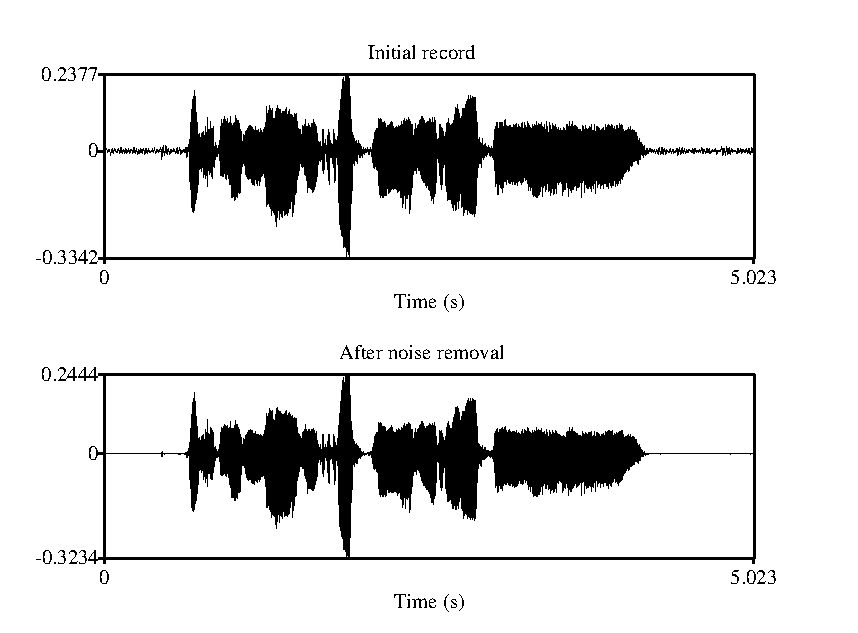
\includegraphics[width=2in]{pict/praat.eps}
\column{.5\textwidth}
\begin{verbatim}
\begin{columns}
\column{.5\textwidth}
% isi kolom1
\column{.5\textwidth}
% isi kolom2
\end{column}
\end{verbatim}
\end{columns}
\end{frame}

\section{4. Memasukkan tema}
\begin{frame}[t,fragile]{Bagaimana menginstall tema Beamer }
\begin{itemize}
\item Install Beamer
  \begin{itemize}
  \item Pada ubuntu: \verb!sudo apt install texlive-latex-extra!
  \item Baca file: tes-beamer
  \end{itemize}
\item Install tema Beamer
  \begin{itemize}
  \item git clone https://github.com/bbatsov/beamer-torino-theme.git
  \item cd beamer-torino-theme.git
  \item sudo cp -r themes /usr/share/texlive/texmf-dist/tex/latex/beamer/
  \item sudo texhash
  \end{itemize}
\item Baca contoh berikut:
  \begin{itemize}
  \item \verb!chameleon.tex!: tema berwarna hijau dengan watermark di pojok kanan bawah.
  \item \verb!nouvelle.tex!: tema berwarna hijau dan merah dengan bullet list bulat
  \item \verb!freewilly.tex!: tema berwarna biru dengan logo dan bullet kotak
  \end{itemize}
\end{itemize}
\end{frame}

\end{document}
